

\tikzset{every picture/.style={line width=0.75pt}} %set default line width to 0.75pt        

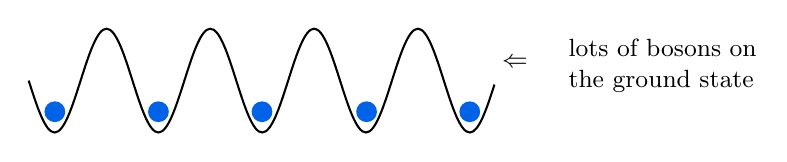
\begin{tikzpicture}[x=0.75pt,y=0.75pt,yscale=-1,xscale=1]
%uncomment if require: \path (0,67); %set diagram left start at 0, and has height of 67

%Shape: Wave [id:dp49770649258615707] 
\draw  [color={rgb, 255:red, 0; green, 0; blue, 0 }  ,draw opacity=1 ] (10,35) .. controls (14.08,47.81) and (17.98,60) .. (22.5,60) .. controls (27.02,60) and (30.92,47.81) .. (35,35) .. controls (39.08,22.19) and (42.98,10) .. (47.5,10) .. controls (52.02,10) and (55.92,22.19) .. (60,35) .. controls (64.08,47.81) and (67.98,60) .. (72.5,60) .. controls (77.02,60) and (80.92,47.81) .. (85,35) .. controls (89.08,22.19) and (92.98,10) .. (97.5,10) .. controls (102.02,10) and (105.92,22.19) .. (110,35) .. controls (114.08,47.81) and (117.98,60) .. (122.5,60) .. controls (127.02,60) and (130.92,47.81) .. (135,35) .. controls (139.08,22.19) and (142.98,10) .. (147.5,10) .. controls (152.02,10) and (155.92,22.19) .. (160,35) .. controls (164.08,47.81) and (167.98,60) .. (172.5,60) .. controls (177.02,60) and (180.92,47.81) .. (185,35) .. controls (189.08,22.19) and (192.98,10) .. (197.5,10) .. controls (202.02,10) and (205.92,22.19) .. (210,35) .. controls (214.08,47.81) and (217.98,60) .. (222.5,60) .. controls (226.8,60) and (230.54,48.98) .. (234.4,36.88) ;
%Shape: Circle [id:dp870205875238355] 
\draw  [draw opacity=0][fill={rgb, 255:red, 0; green, 98; blue, 230 }  ,fill opacity=1 ] (17.6,50) .. controls (17.6,47.24) and (19.84,45) .. (22.6,45) .. controls (25.36,45) and (27.6,47.24) .. (27.6,50) .. controls (27.6,52.76) and (25.36,55) .. (22.6,55) .. controls (19.84,55) and (17.6,52.76) .. (17.6,50) -- cycle ;
%Shape: Circle [id:dp7879328877360514] 
\draw  [draw opacity=0][fill={rgb, 255:red, 0; green, 98; blue, 230 }  ,fill opacity=1 ] (67.5,50) .. controls (67.5,47.24) and (69.74,45) .. (72.5,45) .. controls (75.26,45) and (77.5,47.24) .. (77.5,50) .. controls (77.5,52.76) and (75.26,55) .. (72.5,55) .. controls (69.74,55) and (67.5,52.76) .. (67.5,50) -- cycle ;
%Shape: Circle [id:dp676964482149583] 
\draw  [draw opacity=0][fill={rgb, 255:red, 0; green, 98; blue, 230 }  ,fill opacity=1 ] (117.4,50) .. controls (117.4,47.24) and (119.64,45) .. (122.4,45) .. controls (125.16,45) and (127.4,47.24) .. (127.4,50) .. controls (127.4,52.76) and (125.16,55) .. (122.4,55) .. controls (119.64,55) and (117.4,52.76) .. (117.4,50) -- cycle ;
%Shape: Circle [id:dp5468116419516752] 
\draw  [draw opacity=0][fill={rgb, 255:red, 0; green, 98; blue, 230 }  ,fill opacity=1 ] (167.8,50) .. controls (167.8,47.24) and (170.04,45) .. (172.8,45) .. controls (175.56,45) and (177.8,47.24) .. (177.8,50) .. controls (177.8,52.76) and (175.56,55) .. (172.8,55) .. controls (170.04,55) and (167.8,52.76) .. (167.8,50) -- cycle ;
%Shape: Circle [id:dp3355085376283945] 
\draw  [draw opacity=0][fill={rgb, 255:red, 0; green, 98; blue, 230 }  ,fill opacity=1 ] (217.5,50) .. controls (217.5,47.24) and (219.74,45) .. (222.5,45) .. controls (225.26,45) and (227.5,47.24) .. (227.5,50) .. controls (227.5,52.76) and (225.26,55) .. (222.5,55) .. controls (219.74,55) and (217.5,52.76) .. (217.5,50) -- cycle ;

% Text Node
\draw (236.6,22.85) node [anchor=north west][inner sep=0.75pt]  [font=\small]  {$\Leftarrow $};
% Text Node
\draw (268.6,13.65) node [anchor=north west][inner sep=0.75pt]  [font=\small] [align=left] {lots of bosons on\\the ground state};


\end{tikzpicture}
